\subsection{Redesigning the database model}\label{databaseModelRedesignNF}
We will now create relations describing the new models for the database.
Other groups of the \knox{} pipeline have requested that entities representing articles have a unique Id field, regardless of what is considered good database design.
Similarly, they want a field denoting the total words appearing in the article.

\begin{equation}\label{eq:newDatabaseRelationalModel}
    \begin{split}
        article(\underline{article\_id: \mathbb{Z^+}} title:text,\\ totalwords:\mathbb{Z^+}, publisher\_name \rightarrow publisher), \\
        word(\underline{text:text}),\\
        publisher(\underline{publisher\_name:text}),\\
        occursIn(\underline{text \rightarrow word}, \underline{article\_id \rightarrow article}, count:\mathbb{Z^+})\\
    \end{split}
\end{equation}


Having established these constraints, design have been created using the relational model (equation \ref{eq:newDatabaseRelationalModel}) and the E-R model (figure \ref{fig:newdatabaseRedesignER}).

\begin{figure}[H]
    \centering
    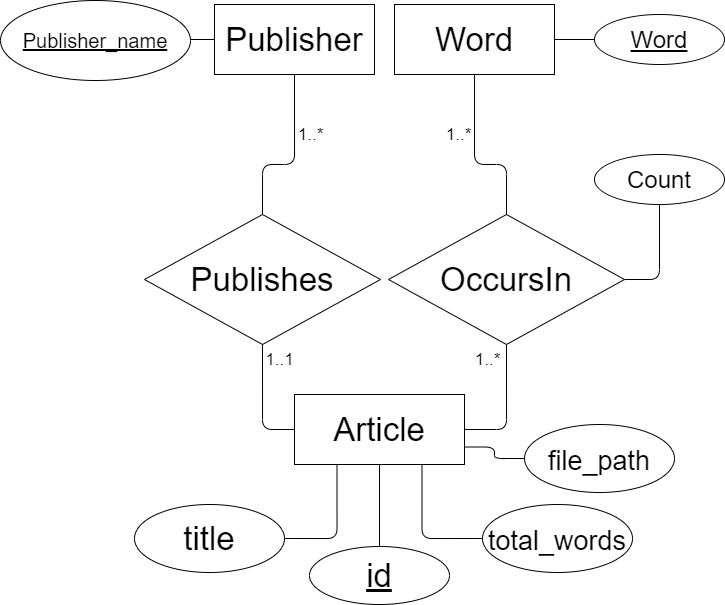
\includegraphics[scale=0.35]{Images/new ER.drawio.png}
    \caption{ER diagram depicting the new model of the database. Notice that the relationship set \textit{Publishes} is not implemented.}
    \label{fig:newdatabaseRedesignER}
\end{figure}